\documentclass[11pt, a4paper]{article}
%\usepackage{proj1}
\usepackage{natbib}
\usepackage{fancyhdr}  
\usepackage{subcaption}
\usepackage{caption}
\usepackage{graphicx}
\usepackage{numprint}
\usepackage{multirow}
\linespread{1.25} 
\setlength{\parindent}{0cm}
\graphicspath{{Images/}}
\usepackage{hyperref}
\usepackage{amsmath}
\usepackage{amsfonts}
\usepackage{amssymb}
\usepackage{amsthm}
\usepackage{mathtools}
\usepackage{commath}
\usepackage{bbm}

%\usepackage[sc,osf]{mathpazo}
\usepackage{subcaption}
\usepackage[a4paper, top=1in, left=1.0in, right=1.0in, bottom=1in, includehead, includefoot]{geometry} %Usually have top as 1in

\usepackage{listings}
\usepackage{color} %red, green, blue, yellow, cyan, magenta, black, white
\definecolor{mygreen}{RGB}{28,172,0} % color values Red, Green, Blue
\definecolor{mylilas}{RGB}{170,55,241}


\hypersetup{colorlinks,linkcolor={black},citecolor={blue},urlcolor={black}}
\usepackage{color}
\urlstyle{same}


\theoremstyle{definition}
\newtheorem{definition}{Definition}[section]

\newcommand{\adja}{q_a}
\newcommand{\adjb}{q_b}
\newcommand{\adjaB}{q_{a,\partial \Omega}}
\newcommand{\adjbB}{q_{b,\partial \Omega}}
\newcommand{\adjB}{q_{\partial \Omega}}
\newcommand{\Adja}{\mathbf{p}}
\newcommand{\Adjb}{q}
\newcommand{\adj}{q}
\newcommand{\Adjc}{{q}_{\partial \Omega}}
\newcommand{\ra}{\rho_a}
\newcommand{\rb}{\rho_b}
\newcommand{\w}{\mathbf{w}}
\newcommand{\f}{\mathbf{f}}
\newcommand{\ve}{\mathbf{v}}
\newcommand{\n}{\mathbf{n}}
\newcommand{\h}{\mathbf{h}}
\newcommand{\K}{\mathbf{K}}
\newcommand{\hr}{\widehat \rho}

%	\begin{figure}[h]
%		\centering
%		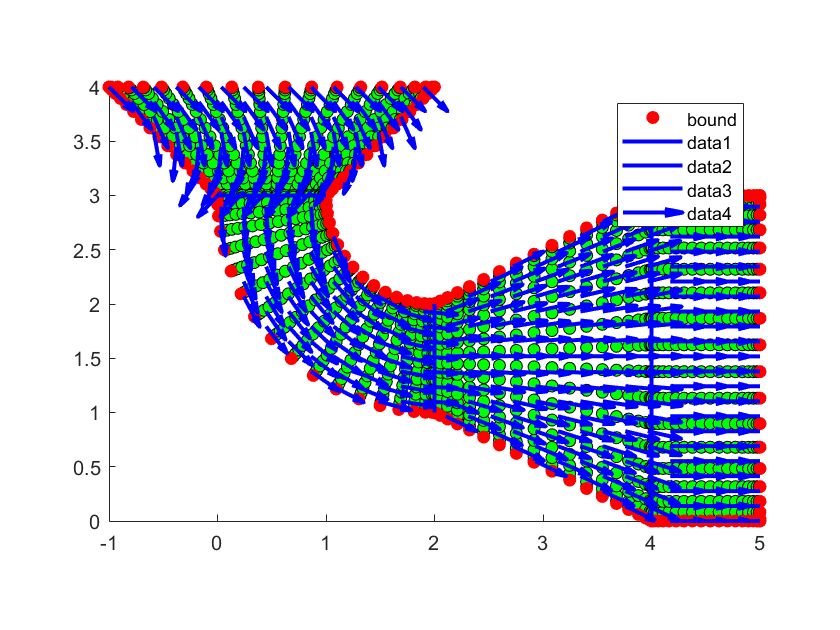
\includegraphics[scale=0.35]{F1.png}
%		\caption{Forward $\rho$ for $a = 0.01$} 
%		\label{F1}
%	\end{figure}

\begin{document}
	
	
\section*{Optimality System of the Averaged Advection Diffusion Equation}
The optimality system is:
\begin{align*}
	\frac{\partial \rho}{\partial t} &= \frac{1}{r} \frac{\partial \rho}{\partial r} +  \frac{\partial^2 \rho}{\partial r^2} + \frac{\partial \rho}{\partial z^2} - \frac{\rho\w_r}{r} - \nabla \cdot (\rho \w ) + f\\
	0 &= \left(- \left(\frac{\partial \rho}{\partial r},  \frac{\partial \rho}{\partial z}\right) + \rho \w \right) \cdot \n \\
	\\
	\frac{\partial q}{\partial t} &= - \frac{1}{r} \frac{\partial q}{\partial r} -  \frac{\partial^2 q}{\partial r^2} - \frac{\partial q}{\partial z^2} - \w \cdot \left(\frac{\partial q}{\partial r},  \frac{\partial q}{\partial z}\right) - \rho + \hr\\
	0 &= \left(\frac{\partial q}{\partial r},  \frac{\partial q}{\partial z}\right) \cdot \n \\
	\\
	\w &= - \frac{1}{\beta}\rho  \left(\frac{\partial q}{\partial r},  \frac{\partial q}{\partial z}\right)
\end{align*}

I used the expanded version of the term in the implementation, where $\nabla$ is defined with respect to $r$ and $z$:
$\nabla \cdot (\rho \w) = \w_r\frac{\partial \rho}{\partial r} + \w_z\frac{\partial \rho}{\partial z} +\rho\frac{\partial \w_r }{\partial r} + \rho\frac{\partial \w_z}{\partial z} $.
\subsection*{Exact Solution}
We are choosing an exact solution which satisfies the boundary conditions, matches the final time condition for $q$ and is invariant in $\theta$. We choose:
\begin{align*}
	\rho &= \beta^{1/2} e^t \cos(\pi r) \cos (\pi z)\\
	q &= \beta^{1/2}(e^T - e^t)\cos(\pi r)\cos(\pi z),
\end{align*}
and use these to determine the values of $\w$, $f$ and $\hr$.


	
\end{document}